% Template for ICIP-2022 paper; to be used with:
%          spconf.sty  - ICASSP/ICIP LaTeX style file, and
%          IEEEbib.bst - IEEE bibliography style file.
% --------------------------------------------------------------------------
\documentclass{article}
\usepackage{algorithm,algpseudocode,bm,spconf,amsmath,graphicx,verbatim}

\title{Maximum Likelihood Multiframe Registration Under Constant Translation}
\name{Evan Widloski and Farzad Kamalabadi\thanks{Thanks to XYZ agency for funding.}}
\address{University of Illinois Urbana-Champaign}

% ------------------- Macros ----------------------
% probability equals sign
\newcommand\peq{\mkern1.5mu{=}\mkern1.5mu}
% likelihood center pipe
\newcommand\lpipe{\mkern1.5mu{|}\mkern1.5mu}


% ------------------- Header ----------------------
\begin{document}
\maketitle
\begin{abstract}
  We present a registration algorithm which jointly estimates motion and the ground truth image from a set of noisy frames under rigid, constant, translation.  With additive white Gaussian noise, the algorithm is optimal in the maximum likelihood sense.  Furthermore, the algorithm is parameterless and non-iterative, requiring a fixed number of operations commonly available on embedded imaging systems such as FFT, multiplication, and downsampling operations which facilitates speed and ease of implementation.  The computation time and accuracy is compared to other algorithms of the same class.  The algorithm outperforms other pairwise or multiframe methods without an explicit motion model, especially in the low SNR regime.
\end{abstract}
%
\begin{keywords}
  registration, maximum likelihood
\end{keywords}
%
%
% ------------------- Introduction ----------------------
\section{Introduction}
\label{sec:introduction}

Image alignment, or image registration is a classic problem in the field of image processing in which an image or image sequence has been transformed from some reference image.
Registration is an important preprocessing step in image processing pipelines involving change detection, image mosaicing, and super-resolution with applications in medical imaging, computer vision tasks, military surveillance, and remote-sensing (cite here).

A wide range of techniques have been developed over the preceding decades, with varying models on the type of motion allowed between frames, content of the scene, changes to objects within the scene, and computational resources available.  In particular we have developed an area-based registration algorithm according to the classification system given in (cite zitova, flusser, brown, etc).

The algorithm is focused on astronomical imaging, where long integration times are sometimes necessary to have sufficient SNR in low light caused by target faintness or low optical efficiency of the imaging system.  However, longer integration times can induce significant motion blur in the images being captured, reducing angular resolution.  Instead, if shorter integration times in a sequence of images can be fused, longer effective integration time can be attained without the associated increase in motion blur.

In particular, the algorithm was conceived for the upcoming VISORS mission, a formation flying cubesat mission studying the solar corona at high resolution (cite Preliminary design of...), where the motion of the scene is approximately constant translation throughout the 10 second capture window.

In the next sections, we provide an observation model describing motion of the frames and noise, a description of the algorithm and suggested implementation for fast computation, a proof of optimality under the described motion and noise model, and experimental results comparing registration error of the algorithm with other multiframe methods.

\begin{figure}[htb]
\begin{minipage}[b]{.48\linewidth}
  \centering
  \centerline{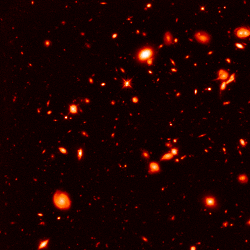
\includegraphics[width=4.0cm]{images/frame_clean.png}}
%  \vspace{1.5cm}
  \centerline{Noiseless frame}\medskip
\end{minipage}
\hfill
\begin{minipage}[b]{0.48\linewidth}
  \centering
  \centerline{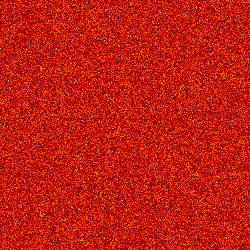
\includegraphics[width=4.0cm]{images/frame.png}}
%  \vspace{1.5cm}
  \centerline{Noisy frame. -30dB SNR}\medskip
\end{minipage}
  \caption{Simulated spacecraft field of view.  False color.}
\label{fig:scene}
\end{figure}


% ------------------- Algorithm ----------------------
\section{Observation Model and Algorithm}
\label{sec:algorithm}

Let $[y_1, ..., y_K]$ be an ordered sequence of $K$ noisy observed frames captured at a constant frame rate with constant drift between frames of $c$ pixels. $c$ is a vector (generally with length 2, corresponding to 2D images).

For each $y_k$, we have

$$y_k = T_{kc}(\mu) + n_k$$

where $T_{kc}$ is a translation operator by vector $kc$ pixels, $\mu$ is a Nyquist sampled version of ground truth scene (also known as the reference image), and $n_k$ is measurement noise.  We have assumed $T$ to be a circular translation for ease of derivation, which holds approximately true for small $c$ relative to the size of a frame.

Note that we have assumed the blurring induced by motion and the imaging system is spatially and temporally invariant, as in the case of adaptive optics and *** (cite gratadour).  Since $T$ is a linear operator, this constant PSF may be integrated entirely into $\mu$ and removed after registration in a separate deconvolution step.

The solution is given by

$$
\hat{c} = \arg \max_c \sum_{m=1}^{K-1}\sum_{k=1}^{K-m} (y_k \ast y_{k+m})[mc]
$$

which consists of a series of correlations, 2 summations, and a downsampling operation.  Taking argmax over the resultant surface yields the maximum likelihood estimate of the motion, $\hat{c}$.

The algorithm can be accelerated by performing correlations in the frequency domain, precomputing the image Fourier transforms with FFT and taking advantage of the linearity of the sum:

\begin{equation}
\hat{c} = \arg \max_c \sum_{m=1}^{K-1} D_m \left[
\mathcal{F}^{-1} \left( \sum_{k=1}^{K-m} Y_k \odot Y_{k+m} \right)
\right]
\label{eq:algorithm}
\end{equation}

where $D_m$ is a downsample operator by $m$ pixels (with zero padding to maintain shape), $\mathcal{F}^{-1}$ is the inverse FFT algorithm, $Y_k$ is the Fourier transform of $y_k$, and $\odot$ is the elementwise product operator.
The algorithm can be broken into 4 steps, shown below and illustrated graphically in Figure \ref{fig:algorithm}:

\begin{enumerate}
  \item Precompute image Fourier transforms:
    $$Y_k=\mathcal{F}(y_k) \text{ for } k=1,...,K$$
  \item Compute image correlations and sum into groups by degree of separation $m$:
    $$S_m = \mathcal{F}^{-1} \left( \sum_{k=1}^{K-m} Y_k \odot Y_{k+m} \right) \text{ for } m=1, ..., K-1$$
  \item Downsample correlation groups by degree of separation and sum:
    $$\sum_{m=1}^{K-1} D_m \left[ S_m \right]$$
  \item Take the argmax of the resultant surface to find the estimate $\hat{c}$
    $$\hat{c} = \arg \max_c \sum_{m=1}^{K-1} D_m \left[ S_m \right]$$
\end{enumerate}

\begin{figure}[htb]
  \begin{minipage}[b]{1\linewidth}
    \centering
    \centerline{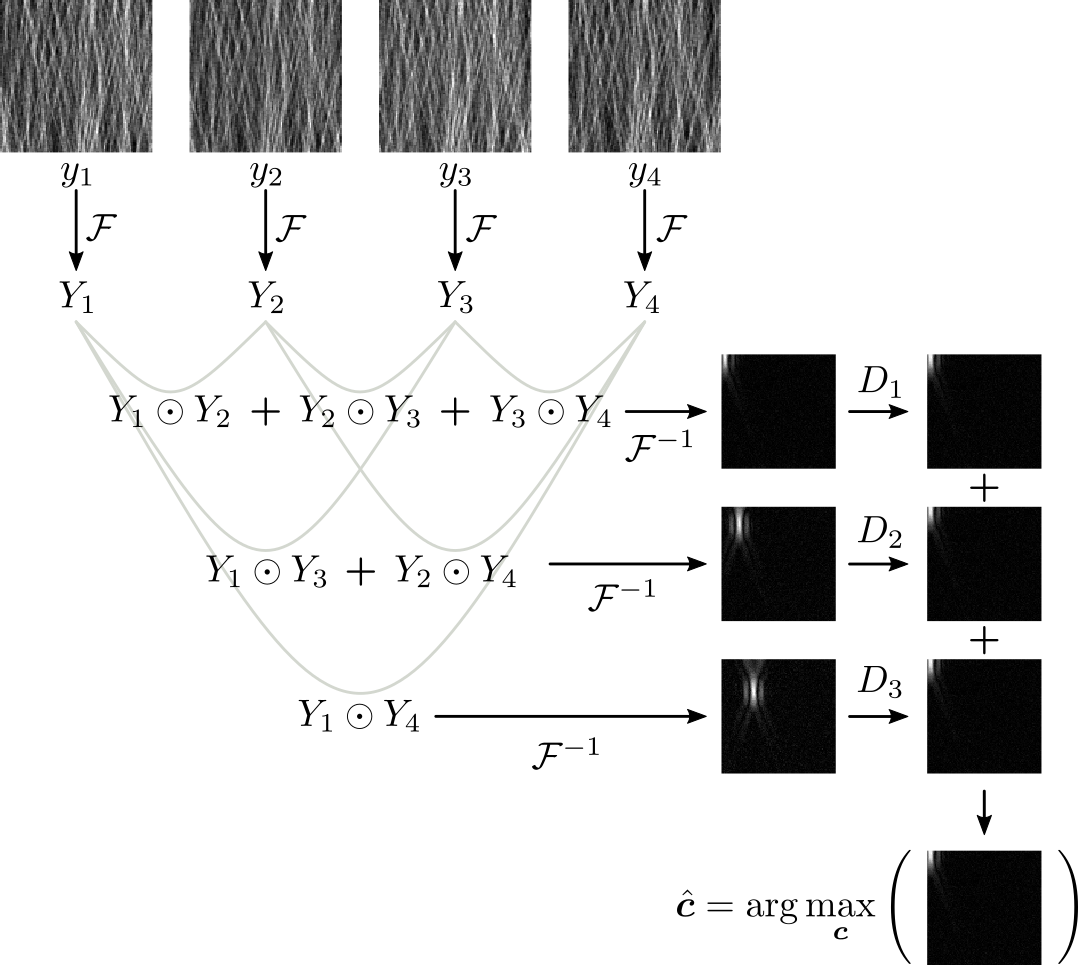
\includegraphics[width=8.5cm]{images/algorithm.png}}
  \end{minipage}
  \caption{Graphical diagram of algorithm given in Equation \ref{eq:algorithm} for a sequence of 4 frames}
  \label{fig:algorithm}
\end{figure}

% ------------------- Optimality ----------------------
\section{Proof of Optimality}
\label{sec:optimality}

The proof of optimality is presented in 3 parts:

\begin{enumerate}
\item Derive expression for likelihood maximization over $c$ and $\mu$
\item Show that most likely value for $\mu$ depends entirely on $c$
\item Show that log-likelihood solution consists of a sum of downsampled cross correlations
\end{enumerate}

Given the previous observation model

$$y_k = T_{kc}(\mu) + n_k$$

assume $n_k \sim \mathcal{N}(0, \sigma^2)$ is additive white Gaussian noise with variance $\sigma^2$.  Without loss of generality, we assume the observed frames to be one dimensional vectors of length $N$. ***(FIXME: summation offset)

The log-likelihood of having a particular $c$ and $\mu$ given an observation sequence is

\begin{align}
  \hat{c}, \hat{\mu} &= \arg \max_{c, \mu} \ln \mathcal{L}(c, \mu \lpipe y_1, ..., y_K) = \ln \prod_{k=1}^K \mathcal{L}(c, \mu \lpipe y_k) \nonumber \\
  &=\arg \max_{c, \mu} \ln \prod_{k=1}^K \prod_{n=1}^N \mathcal{L}(c, \mu \lpipe y_{k,n}) \nonumber \\
  &=\arg \max_{c, \mu} \ln \prod_{k=1}^K \prod_{n=1}^N \frac{1}{\sigma^2 \sqrt{2 \pi}} \text{exp} \left[- \frac{(y_{k,n} - T_{kc}(\mu)_n)^2}{\sigma^2}\right] \nonumber \\
  &=\arg \min_{c, \mu} \sum_{k=1}^K \sum_{n=1}^N (y_{k,n} - T_{kc}(\mu)_n)^2 \label{eqn:min}
\end{align}

To show that the value of $\mu$ with maximum likelihood depends only on $c$, we will take the derivative of the expression being minimized with respect to the jth element of $\mu$.  Due to the circular nature of $T$, some modular arithmetic is necessary, denoted by operator $\%$.

\begin{align*}
  &\frac{d}{d\mu_j}\left[\sum_{k=1}^K \sum_{n=1}^N (y_{k,n} - T_{kc}(\mu)_n)^2\right] = 0 \\
  &=\sum_{k=1}^K \sum_{n=1}^N \frac{d}{d\mu_j}\left[(y_{k,n} - \mu_{kc + n \% N})^2\right] = 0 \\
  &=\sum_{k=1}^K \frac{d}{d\mu_j}\left[(y_{k,j - kc \% N} - \mu_j)^2\right] = 0 \\
  &=\sum_{k=1}^K \frac{d}{d\mu_j}\left[(T_{-kc}(y_k)_j - \mu_j)^2\right] = 0 \\
  &=\sum_{k=1}^K -2(T_{-kc}(y_k)_j - \mu_j) = 0 \\
  &\Longrightarrow \mu_j = \sum_{k=1}^K T_{-kc}(y_k)_j \\
  &\Longrightarrow \mu = \sum_{k=1}^K T_{-kc}(y_k)
\end{align*}

This is simply the sum of the motion corrected noisy frames.  Plugging this into Equation \ref{eqn:min}, we can see that the minimization over $\mu$ can be dropped.  Expanding an eliminating constant terms, we get

\begin{align*}
\end{align*}


\newpage
.
\newpage

% ------------------- Experimental Results ----------------------
\section{Experimental Results}
\label{sec:results}

\begin{figure}[htb]
\begin{minipage}[b]{.48\linewidth}
  \centering
  \centerline{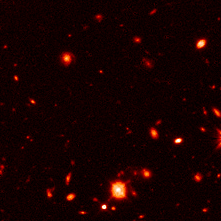
\includegraphics[width=4.0cm]{images/recon_clean.png}}
%  \vspace{1.5cm}
  \centerline{Ground truth}\medskip
\end{minipage}
\hfill
\begin{minipage}[b]{0.48\linewidth}
  \centering
  \centerline{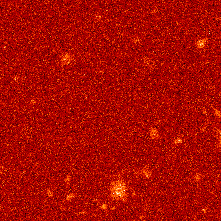
\includegraphics[width=4.0cm]{images/recon.png}}
%  \vspace{1.5cm}
  \centerline{Reconstruction}\medskip
\end{minipage}
  \caption{Reconstruction result for -30dB SNR and $K=30$ frames.}
\label{fig:scene}
\end{figure}

\begin{figure}[htb]
  \begin{minipage}[b]{1\linewidth}
    \centering
    \centerline{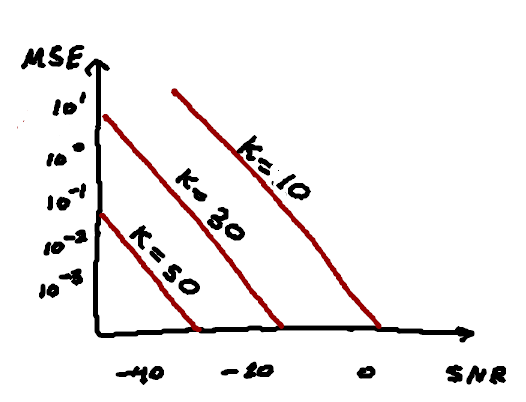
\includegraphics[width=8.5cm]{images/mse.png}}
  \end{minipage}
  \caption{(placeholder***) Registration MSE for various observation SNRs and number of frames $K$.}
  \label{fig:mse}
\end{figure}

% ------------------- Experimental Results ----------------------
\section{Relation to Prior Work}
\label{sec:prior}

The text of the paper should contain discussions on how the paper's
contributions are related to prior work in the field. It is important
to put new work in  context, to give credit to foundational work, and
to provide details associated with the previous work that have appeared
in the literature. This discussion may be a separate, numbered section
or it may appear elsewhere in the body of the manuscript, but it must
be present.

You should differentiate what is new and how your work expands on
or takes a different path from the prior studies. An example might
read something to the effect: "The work presented here has focused
on the formulation of the ABC algorithm, which takes advantage of
non-uniform time-frequency domain analysis of data. The work by
Smith and Cohen considers only fixed time-domain analysis and
the work by Jones et al takes a different approach based on
fixed frequency partitioning. While the present study is related
to recent approaches in time-frequency analysis [3-5], it capitalizes
on a new feature space, which was not considered in these earlier
studies."


% ------------------- Future Work ----------------------
\section{Future Work}
\label{sec:future}

% ------------------- Future Work ----------------------
\section{Conclusion}
\label{sec:future}

\vfill\pagebreak

\section{REFERENCES}
\label{sec:refs}

List and number all bibliographical references at the end of the
paper. The references can be numbered in alphabetic order or in
order of appearance in the document. When referring to them in
the text, type the corresponding reference number in square
brackets as shown at the end of this sentence . An
additional final page (the fifth page, in most cases) is
allowed, but must contain only references to the prior
literature.

% References should be produced using the bibtex program from suitable
% BiBTeX files (here: strings, refs, manuals). The IEEEbib.bst bibliography
% style file from IEEE produces unsorted bibliography list.
% -------------------------------------------------------------------------
%% \bibliographystyle{IEEEbib}
%% \bibliography{strings,refs}

\end{document}
